\section{Introduction}
    \label{s:intro}
    The number of analysis tools required in multidisciplinary design optimization (MDO) studies is growing
    in parallel with the increasing scope of typical problems. An example can
    be observed in the historical evolution of the disciplines involved in MDO problems in aircraft design.
    Multidisciplinary optimization emerged as a separate field from structural optimization through the
    need to introduce formal techniques for managing the coupling of aerodynamic loads and structural
    deformations, through the linking of aerodynamic vortex lattice or panel methods with structural finite
    element models \cite{Cramer1994}. Subsequently, flight performance and life cycle economics tools were integrated
    into MDO analysis workflows for conceptual and preliminary design studies \cite{Sobieski1998}. Currently, MDO
    problems for aircraft design also often include tools for aircraft noise and emissions. In sum, it is now
    commonplace for 5--10 analysis tools to be employed for typical aircraft design optimization studies.
    
    The number of analysis tools is expected to grow in the future as the scope of MDO problems continues
    to evolve, and as computing is increasingly commoditized. This expansion of scope will be driven, in
    part, by consideration of additional disciplines. Current trends on the horizon for aircraft MDO studies
    include incorporation of manufacturing analyses \cite{deWeck2007}, subsystem performance \cite{Dean2009,Gavel2006}, and models of emissions, noise, or economics \cite{Antoine2004,Rallabhandi2007,Kirby2008}.

    The time and expense for setting up 
    analysis models is growing in conjunction with the increasing scope of MDO problems. 
    Multidisciplinary Design Analysis and Optimization (MDAO)
    frameworks such as OpenMDAO\cite{Gray2012} and {ModelCenter}\textregistered have enabled a new level of analysis tool integration 
    and have paved the way for models with more analyses and increasing numbers of interdisciplinary couplings. This 
    new capability has created a new challenge. Even models with tens of analyses could include hundreds or thousands
    of variables that are interdependent and must be linked in the framework. 
    A common situation is that different analyses provide differing values for the 
    same physical quantity, and these conflicts need to be resolved. These differing values 
    may not even be in the same format. These occurrences are particularly acute when analysis tools have differing fidelities. For
    example, an abstracted aerodynamic analysis such as an empirical drag buildup model may return only
    integrated drag, whereas a CFD tool may return pressure and shear stress distributions across the entire
    surface grid. If an analysis downstream of the aerodynamics tool needs only integrated drag as an input,
    then the designer has a free choice of which of the two possible aerodynamics analysis tools to select to
    provide the drag estimate (presuming that drag can be computed from surface distributions by a simple
    integration algorithm). On the other hand, if a downstream analysis needs a pressure distribution in
    order to compute pitching moment, for example, then any feasible MDO problem formulation must
    include CFD or similar analysis in the data flow, regardless of whether the empirical drag buildup model
    is also included.

    With the added complexity from larger models, it is plausible that the task of combining all the analyses into a 
    consistent system model capable of solving a relevant engineering design 
    problem could approach the cost and time requirements of creating any of the discipline 
    analyses themselves. For these large scale MDO problems, the couplings between the 
    analyses begin to dominate the effort required in setting up the model. It is this problem of 
    determining sets of analysis tools and their interconnectivities to form realistic
    multidisciplinary problems that is the subject of this paper. We are motivated by the following notional
    but realistic problem of organizing an MDO study for a complex system:

    \begin{quote}
    A new system is being designed for which there is little or no historical precedent. The system
    is complex, as measured by the number of coupled disciplines and/or components involved in the
    analysis. A general optimization problem statement has been formulated based on system-level objectives and constraints; however, it is unclear which engineering analysis tools should
    be interconnected in order to solve the optimization problem. A team of disciplinary and/or component design engineers has been formed in which each engineer has expertise in a
    particular analysis tool or component model. The engineers meet to discuss the approach to
    interconnecting their tools to achieve the required system-level MDO model.
    \end{quote}

    Our goal is to develop formalism for expressing analysis interconnectivity and for determining feasible
    data flows to assist an engineering team conducting this task. Because the problem deals with
    interconnectivity, we base our approach on the representations and techniques of graph theory. The 
    proposed graph syntax is closely related to the REMS system proposed by 
    Alexandrov and Lewis\cite{alexandrov2004}. The approach taken here should be viewed as an extention 
    of the concepts proposed in REMS with the goal of allowing the graphs to more closely interact with 
    existing design processes and MDAO frameworks. 

The approach begins by 
    constructing the \emph{maximal connectivity graph (MCG)} describing all possible
    interconnections between the analysis tools proposed by the engineers. Graph operations are then
    conducted to reduce the MCG down to a \emph{fundamental problem graph (FPG)} that describes the set of analysis
    tools needed to solve the specified system-level design problem.
    Any particular solution procedure for the problem; any relevant MDO solution architecture, e.g. MDF,
    IDF, CO, BLISS, could be selected \emph{post facto} to implement the system-level optimization by
    constructing a \emph{problem solution graph (PSG)} and the corresponding problem solution approach.
    The concept of the FPG and the identification of feasible FPGs are the main contributions of the paper.

    The paper is organized as follows. First, we describe the differences between a fundamental problem
    formulation, which is based only on the system-level optimization problem statement that the
    engineers desire to solve and on the available analysis tools, and a specific problem formulation, which
    additionally presumes a specific MDO solution approach to the problem. Next, we survey the literature in applying
    graph theoretic and formal language approaches to multidisciplinary design problem formulation. 
    We then discuss our graph syntax and representation of MDO problems and describe the procedures for 
    determining the MCG and FPG. Finally, we present an example problem based on an MDO analysis of a 
    commercial aircraft and discuss additional applications enabled by our approach.

\section{Motivation}
\subsection{Specific vs Fundamental Problem Formulation }
	\label{s:specific vs fundamental}
    The Fundamental Problem Formulation (FPF) is our terminology for a 
    statement of the overall system-level optimization problem that does not 
    depend on the choice of solution-specifc elements such as the MDAO 
    framework, optimization algorithm, iterative solver, or execution sequence
    used to solve the problem. The FPF contrasts with problem statements that are written without 
    reference to a specific solution strategy, but that still imply a specific execution sequence.
    For example, consider the Sellar test problem \cite{AIAA:sellar}, with an FPF given as follows:

    \begin{align}
        \txt{given} & \ \ y_1 = D_1(x_1,y_2,z_1,z_2) \notag
        \\      & \ \ y_2 = D_2(y_1,z_1,z_2) \notag
        \\\txt{min.} &\ \ F(x_1,y_1,y_2,z_2) \notag
        \\\txt{w.r.t.} & \ \ x_1,y_1,y_2,z_1,z_2 \notag
        \\\txt{s.t.} & \ \ G_1(y_1) \geq 0 \notag
        \\     & \ \ G_2(y_2) \geq 0
        \label{eqn:simple_fpf}
    \end{align}

    
    In Eq. \ref{eqn:simple_fpf}, $y_1$ is an output of $D_1$ as well as an input 
    to $D_2$. Similarly, $y_2$ is an output of $D_2$ as well as an input 
    to $D_1$. This implies that $D_1$ and $D_2$ are coupled together by means 
    of their reciprical dependence. However no information is given as to weather
    $D_1$ or $D_2$ should be run before the other. Given Eq \ref{eqn:simple_fpf}, 
    it would be equally valid to run $D_1$ first, $D_2$ first, or both simultaneously. 

    Eq. \ref{eqn:simple} gives a modified problem formulation where $D_1$ is run 
    first. A new variable is introduced, $\hat{y_2}$, to break the dependence of
    $D_1$ on $D_2$. Also a new coupling constraint, $H$, to enforce the consistency
    that would otherwise be lost due to $\hat{y_2}$. Equation \ref{eqn:simple} is 
    a specific alternative expression of the more fundamental problem description 
    given in Eq. \ref{eqn:simple_fpf}.

    \begin{align}
        \txt{given} & \ \ y_1 = D_1(x_1,\hat{y_2},z_1,z_2) \notag
        \\      & \ \ y_2 = D_2(y_1,z_1,z_2) \notag
        \\\txt{min.} &\ \ F(x_1,y_1,y_2,z_2) \notag
        \\\txt{w.r.t.} & \ \ x_1,y_1,\hat{y_2},z_1,z_2 \notag
        \\\txt{s.t.} & \ \ H(y_2,\hat{y_2}) = 0 \notag 
        \\     & \ \ G_1(y_1) \geq 0 \notag
        \\     & \ \ G_2(y_2) \geq 0
        \label{eqn:simple}
    \end{align}


\subsection{Existing Graph-Based Syntax}
	\label{s:existing syntax}
    As indicated in the examples in Sec.~\ref{s:specific vs fundamental}, the mathematical 
    language for specifying problem formulations is very general and can be used both for 
    fundamental and specific problem formulations. Tedford and Martins used this mathematical syntax to specify the 
    FPF for a set of test problems and also to describe specific formulations for solving them with a 
    number of optimization architectures\cite{Tedford2009}. Their work demonstrates how multiple specific 
    problem formulations can relate to a common FPG. The challenge with this 
    traditional mathematical syntax is that it is not easily manipulated or analyzed. 

    A number of graph-based methods have been used successfully to translate the 
    mathematical syntax into a more useful computational form. 
    Steward's Design Structure Matrix (DSM) is a square adjacency matrix which captures the relationship between analysis tools.
    Off-diagonal elements of the matrix indicate coupling\cite{Steward1981}. Since a DSM describes a square adjacency matrix, 
    it can be represented in an equivalent directed graph in which nodes represent analysis tools and 
    edges represent information dependence between those tools. The ordering of elements in a DSM can be used to indicate 
    execution order.  For more complex problems, choosing the proper order to run analysis tools is a challenging task. 
    Rogers et al.~developed DeMAID to manipulate a DSM to find an ordering for analysis tools that 
    reduces the cost of solving highly coupled systems\cite{rogers1996,rogers1996demaid}. This re-ordering is done through 
    row operations on the DSM matrix and yields multiple specific problem 
    formulations which all solve the same FPF. 
    
    A DSM by itself is insufficient to describe complete problem formulations because it 
    captures only information about data dependency between analyses; objective and 
    constraint information is missing from the DSM description of the problem. 
    An alternative matrix-based syntax, called a Functional Dependency Table (FDT), was proposed by Wagner and Papalambros. 
    FDT represents the relationship between functions, including objectives and constraints, and specific variables that affect 
    them\cite{Wagner1993}. Similar to DSM, FDT also describes an adjacency matrix of a graph. Unlike the DSM graph, 
    however, the FDT graph is undirected and nodes can represent analysis tools, objectives, 
    or constraints. Edges between nodes represent a dependence on the same 
    variable. Michelena and Papalambros made use of the FDT to solve a graph partitioning problem that yielded 
    more efficient optimization problem decompositions\cite{Michelena1997}. While FDT succeeds at capturing the 
    information about objectives and constraints, its lack of directed edges 
    implies that it cannot capture the coupled data dependency that a DSM captures. 
    The FDT in Fig. \ref{fig:FDT_simple} shows that $D_1$ is dependent on $y_2$ and 
    that $D_2$ is dependent on $y_1$, but you can not infer their coupled dependence from 
    that information alone. This missing information implies 
    that, while FDT is very useful for partitioning problems, it is also not 
    sufficient to completely describe a problem formulation. 
    \begin{figure}[htb!]
        \begin{center}
        \begin{tabular}{|c|c|c|c|c|c|c|}
            \hline
                   & $x_1$ & $y_1$ & $y_2$ & $z_1$ & $z_2$ \\ \hline
            $D_1$  & 1     &       & 1     & 1     & 1     \\ \hline
            $D_2$  &       & 1     &       & 1     & 1     \\ \hline
            $F$    & 1     & 1     & 1     &       & 1     \\ \hline
            $G_1$  &       & 1     &       &       &       \\ \hline
            $G_2$  &       &       & 1     &       &       \\
            \hline
        \end{tabular}
        \caption{Functional Dependency Table (FDT) for Eq. \ref{eqn:simple_fpf} \label{fig:FDT_simple}}
        \end{center}
    \end{figure}

    Alexandrov and Lewis introduced a graph based syntax called REMS which 
    incorporates objectives and constraints into a graph, effectively combining 
    FDT and DSM\cite{alexandrov2004}. REMS retains the square adjacency 
    matrix form from DSM, but by adding the objectives and constraints, it partially 
    combines a traditional DSM with an FDT. This formulation allows REMS to represent data 
    dependency between multiple analysis tools as well as between analysis tools and
    objective/constraint functions. Additionaly, REMS address the need to be able to 
    transition between multiple solution strategies while keeping a constant 
    graph representation of the fundamental problem formulation. REMS provides
    syntax for variables and functions but does not facilitate inclusion 
    of solvers or optimizers in the graph. 

    Lamb and Martins also included objectives and constraint functions as nodes 
    in an Extended DSM (XDSM) in order to capture a more complete description 
    of solution strategies for MDAO problems\cite{Lambe2012}. Unlike REMS, 
    XDSM also includes nodes for solvers and optimziers to enable complete 
    definition of MDAO architectures. Martins uses XDSM to describe 13 different 
    optimization architectures in a survey paper that provides a novel 
    classification of the different techniques \cite{Lambe2011}. With the 
    additional information included in an XDSM, Lu and Martins applied both 
    ordering and partitioning algorithms on an MDAO test problem termed the 
    Scalable Problem \cite{Lu2012}. 

    \begin{figure}
        \begin{center}
        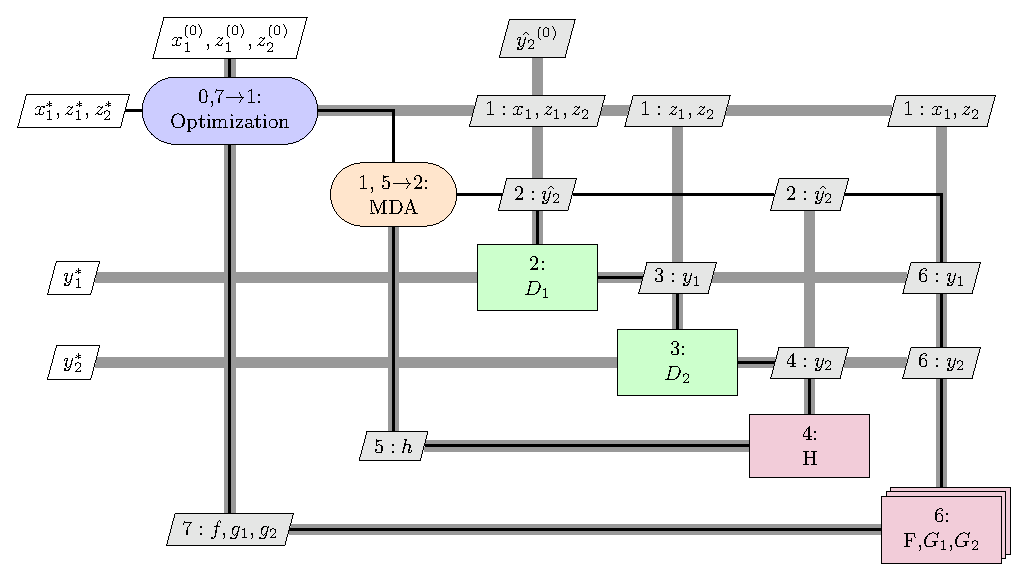
\includegraphics[height=.25\textheight]{XDSM/simple}
        \caption{XDSM for Eq. \ref{eqn:simple}, with a Gauss-Seidel iteration 
          and MDF solution architecture. \label{fig:XDSM_simple}}
        \end{center}
    \end{figure}

    Although XDSM captures many of the functional aspects of FDT, it 
    requires the use of solver and optimizer blocks to represent 
    the relationship between design variables and objectives/constraints. 
    By introducing solver or optimizer blocks, XDSM automatically implies a strategy. 
The XDSM for Eq. \ref{eqn:simple} is 
    given in Figure \ref{fig:XDSM_simple}. This diagram is shown with an 
    assumed Gauss-Seidel iteration scheme and an MDF solution architecture. 

    Of these methods, REMS can describe most aspects of a fundamental 
    problem formulation, but lacks the ability to represent optimizers and 
    solvers in more specific problem formulations. XDSM relies on the provision of  
    optimizers and constraints and is not formulated  
    for a more fundamental problem statement. We propose a new graph syntax that 
    combines the relevant features of REMS and XDSM while retaining the flexiblity to 
    represent a fundamental problem formulation free of solution specific information. 

\subsection{Requirements for a New Graph Syntax}
  \label{s:requirements}
  The goal of the new graph-based syntax presented here is to enable the general structure of an MDAO problem to be described independently of any solution information, 
  while still being able to accomodate the more specific case when a solution 
  strategy is applied. In order to achieve this goal, 
  the graph syntax needs to accomodate a number of MDAO problem constructs: 
  \begin{itemize}
    \item Analysis tools and their interconnections
    \item Design variables, objectives, and constraints
    \item Local and global information
    \item Coupling between analyses
    \item Multi-fidelity analyses
  \end{itemize}

  The new syntax is intended to represent three phases of the design problem 
  formulation process. In the initial problem definition phase, the specific 
  analysis tools and design goals are identified. Next, a single formal problem 
  formulation is identified that specifies design variables, constraints, 
  objectives, analysis tools, and all other elements required to represent 
  the overall MDAO problem. Lastly, a specific procedure for solving the problem 
  is selected, e.g. selecting an MDAO optimization architecture. Using 
  the proposed graph syntax, these phases can be represented with the following 
  three graphs:
  \begin{itemize}
    \item Maximal Connectivity Graph (MCG)
    \item Fundamental Problem Graph (FPG)
    \item Problem Solution Graph (PSG)
  \end{itemize}

  The \emph{maximal connectivity graph} represents the first phase of the problem formulation with all 
  analysis tools being considered and all possible connections between them also present. The second graph 
  is the \emph{fundamental problem graph}, which is comprises only the analyses participating to solve the problem. Finally, a \emph{problem solution graph} 
  may be represented by including additional edges and nodes to represent the 
  solution strategy being employed to solve the problem. This paper focuses on the MCG and FPG and does not describe the PSG in detail.

  The relationship between these three graphs is depicted in Figs.~\ref{f:tree} and \ref{f:hourglass}. 
  The tree diagram demonstrates the fact that it is generally possible to obtain 
  multiple FPGs from a single maximal connectivity graph. The multiple FPGs may correspond to 
  different down-selections of analysis tools, different connections between the tools, 
  or both. Each down-selection shrinks the number of possible FPGs that could be reached 
  until only one remainins. For a given FPG, different PSGs may be obtained by implementing 
  different solution strategies. Considering the size of a graph to be the sum of all of its
  edges and nodes, the hourglass shape in Fig. \ref{f:hourglass} qualitatively illustrates how
  the FPG is obtained from the MCG by \emph{removing} nodes and edges, 
  and the PSG is obtained from the FPG by \emph{adding} nodes and edges.
  \begin{figure}[htb!]
    \centering
    \subfigure[number of possible graphs]{
    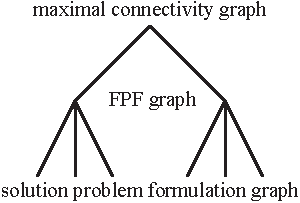
\includegraphics[width=1.75in]{images/tree}
    \label{f:tree}
    }
    \subfigure[graph size]{
    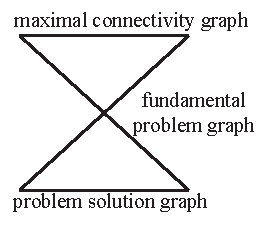
\includegraphics[width=1.75in]{images/hourglass}
    \label{f:hourglass}
    }
  \caption{The relationship between the MCG, FPG, and PSG.}
  \end{figure}